There are two steps to run a kernel on an FPGA (as with any ahead-of-time compilation accelerator):\par

\begin{enumerate}
	\item Compiling the source to a binary which can be run on our hardware of interest
	\item Selecting the correct accelerator that we are interested in at runtime
\end{enumerate}

To compile kernels so that they can run on FPGA hardware, we can use the command line:\par

\begin{tcolorbox}[colback=white,colframe=black]
dpcpp -fintelfpga my\_source\_code.cpp -Xshardware
\end{tcolorbox}

This command tells the compiler to turn all kernels in my\_source\_code.cpp into binaries that can run on an Intel FPGA accelerator and then to package them within the host binary that is generated. When we execute the host binary (e.g., by running ./a.out on Linux), the runtime will automatically program any attached FPGA as required, before executing the submitted kernels, as shown in Figure 17-8.\par

\hspace*{\fill} \par %插入空行
Figure 17-8. FPGA programmed automatically at runtime
\begin{center}
	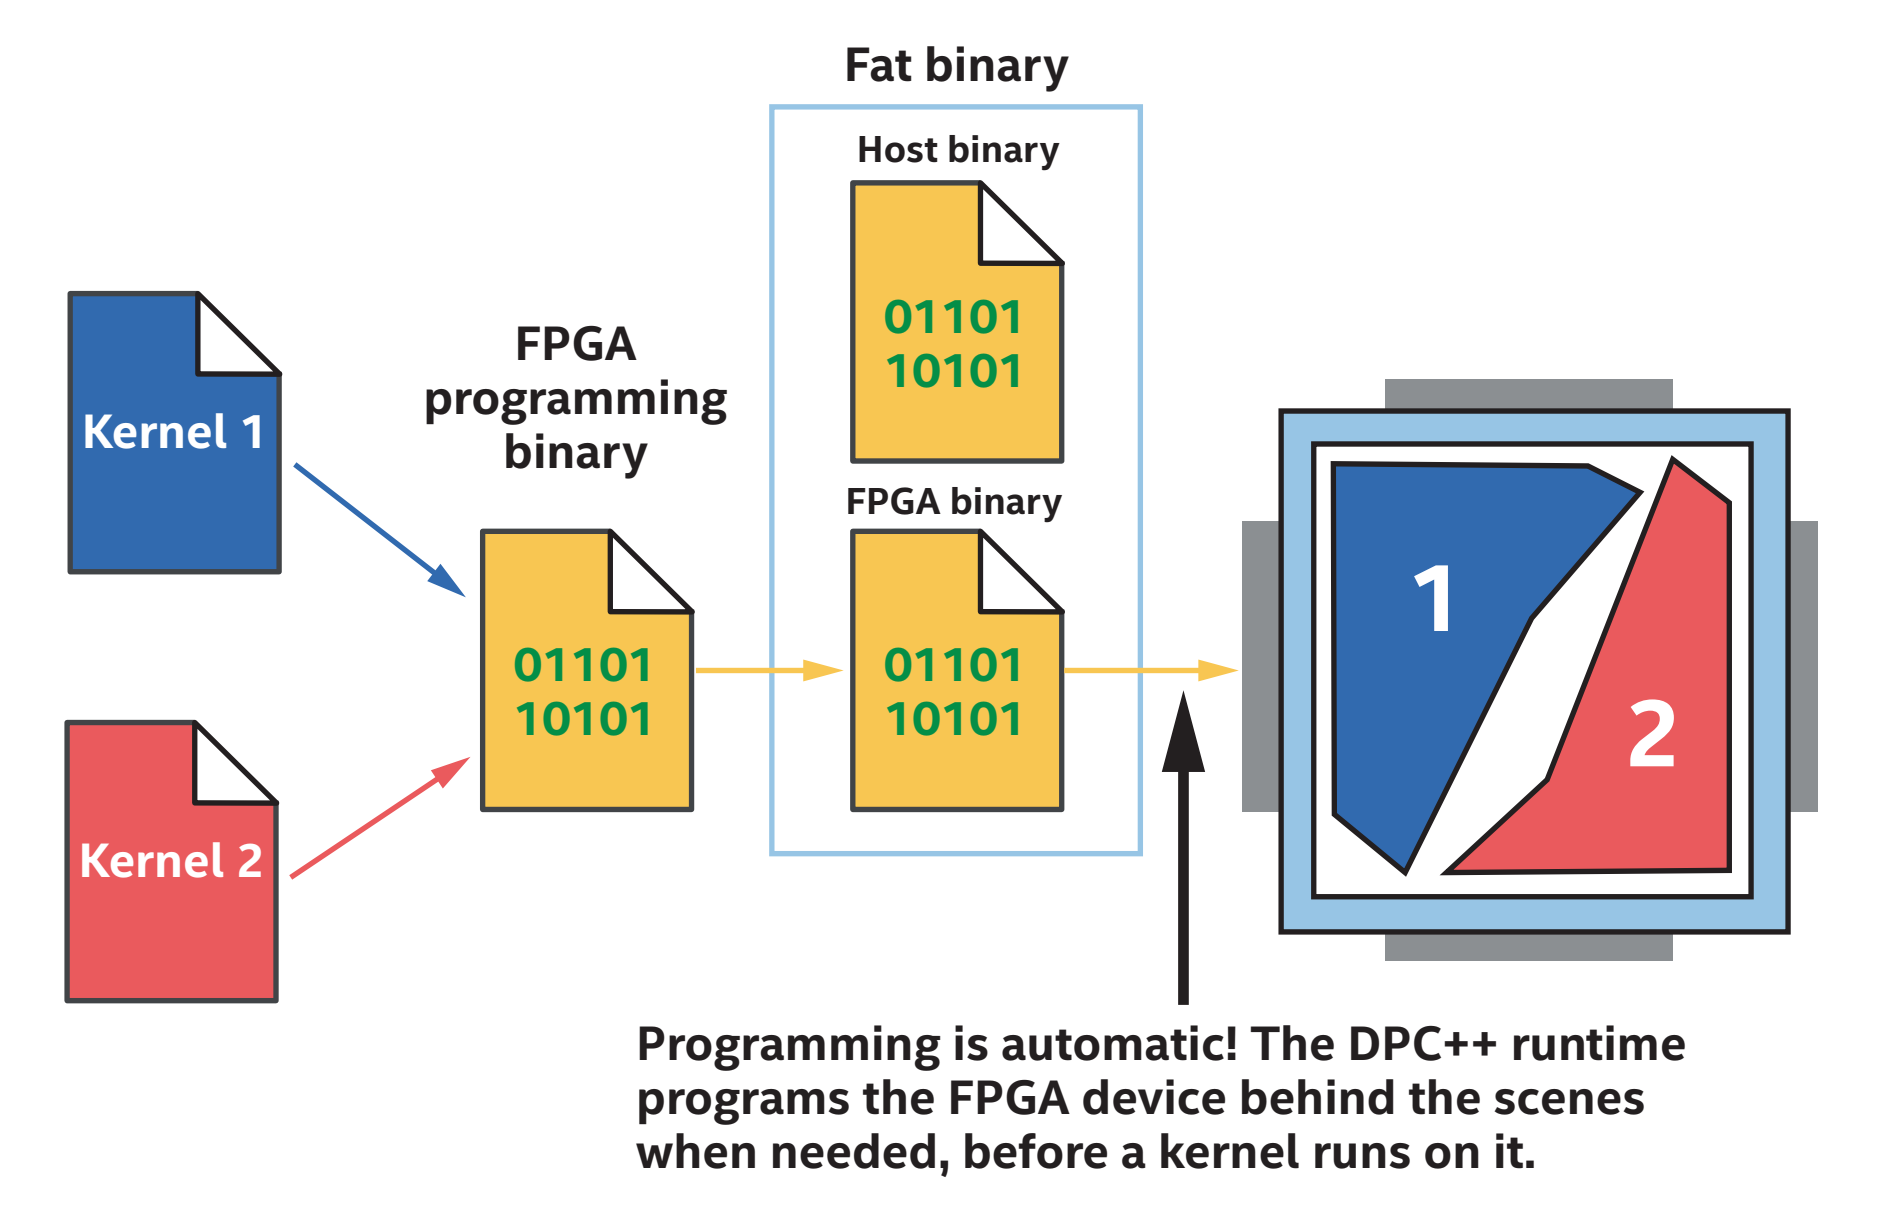
\includegraphics[width=1.0\textwidth]{content/chapter-17/images/9}
\end{center}

\begin{tcolorbox}[colback=red!5!white,colframe=red!75!black]
FPGA programming binaries are embedded within the compiled DPC++ executable that we run on the host. The FPGA is automatically configured behind the scenes for us.\\
When we run a host program and submit the first kernel for execution on an FPGA, there might be a slight delay before the kernel begins executing, while the FPGA is programmed. Resubmitting kernels for additional executions won’t see the same delay because the kernel is already programmed to the device and ready to run.
\end{tcolorbox}

Selection of an FPGA device at runtime was covered in Chapter 2. We need to tell the host program where we want kernels to run because there are typically multiple accelerator options available, such as a CPU and GPU, in addition to the FPGA. To quickly recap one method to select an FPGA during program execution, we can use code like that in Figure 17-9.\par

\hspace*{\fill} \par %插入空行
Figure 17-9. Choosing an FPGA device at runtime using the fpga\_selector
\begin{lstlisting}[caption={}]
#include <CL/sycl.hpp>
#include <CL/sycl/intel/fpga_extensions.hpp> // For fpga_selector
using namespace sycl;

void say_device (const queue& Q) {
	std::cout << "Device : "
			  << Q.get_device().get_info<info::device::name>() 
			  << "\n";
}

int main() {
	queue Q{ INTEL::fpga_selector{} };
	say_device(Q);
	
	Q.submit([&](handler &h){
		h.parallel_for(1024, [=](auto idx) {
			// ...
		});
	});

	return 0;
}
\end{lstlisting}

\hspace*{\fill} \par %插入空行
\textbf{Compile Times}

Rumors abound that compiling designs for an FPGA can take a long time, much longer than compiling for ISA-based accelerators. The rumors are true! The end of this chapter overviews the fine-grained architectural elements of an FPGA that lead to both the advantages of an FPGA and the computationally intensive compilation (place-and-route optimizations) that can take hours in some cases.\par

The compile time from source code to FPGA hardware execution is long enough that we don’t want to develop and iterate on our code exclusively in hardware. FPGA development flows offer several stages that minimize the number of hardware compilations, to make us productive despite the hardware compile times. Figure 17-10 shows the typical stages, where most of our time is spent on the early steps that provide fast turnaround and rapid iteration.\par

\hspace*{\fill} \par %插入空行
Figure 17-10. Most verification and optimization occurs prior to lengthy hardware compilation
\begin{center}
	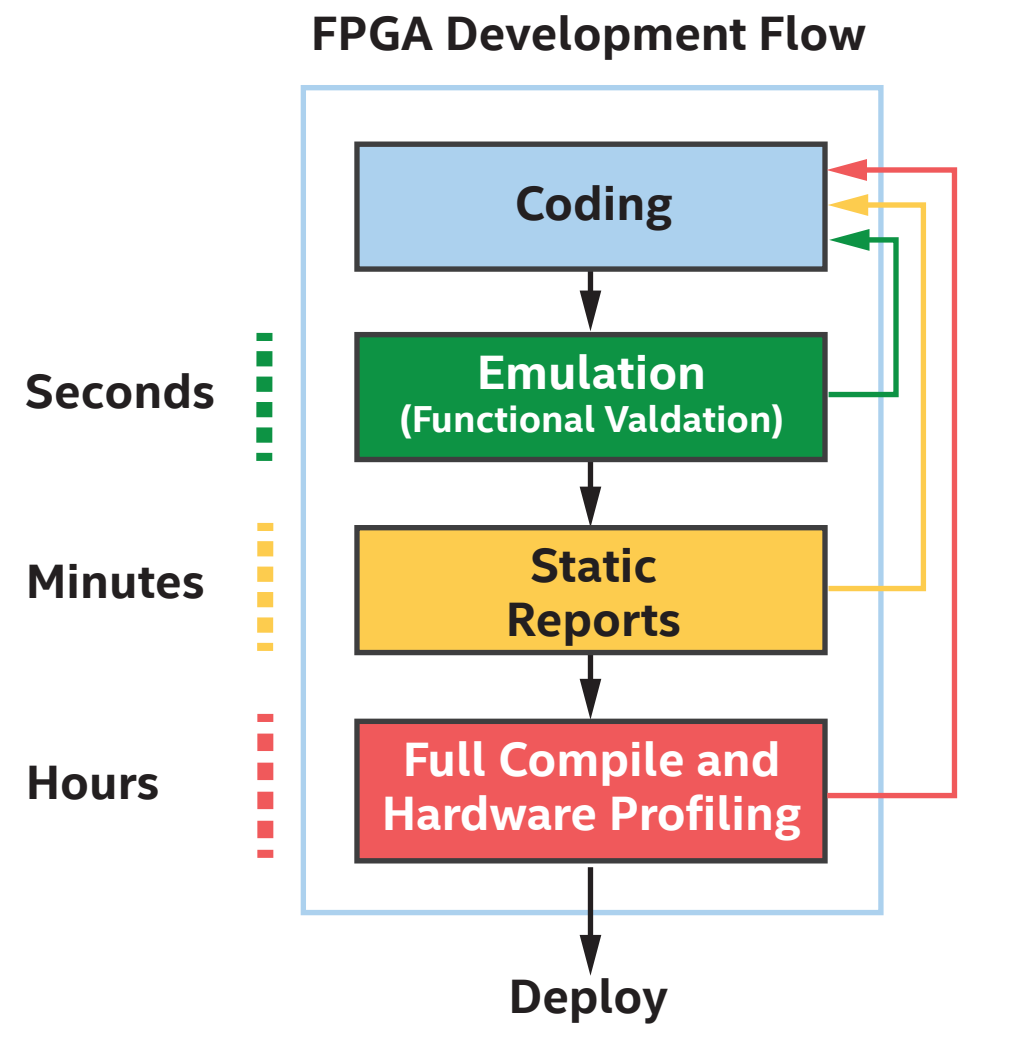
\includegraphics[width=1.0\textwidth]{content/chapter-17/images/10}
\end{center}

Emulation and static reports from the compiler are the cornerstones of FPGA code development in DPC++. The emulator acts as if it was an FPGA, including supporting relevant extensions and emulating the execution model, but runs on the host processor. Compilation time is therefore the same as we would expect from compilation to a CPU device, although we won’t see the performance boost that we would from execution on actual FPGA hardware. The emulator is great for establishing and testing functional correctness in an application.\par

Static reports, like emulation, are generated quickly by the toolchain. They report on the FPGA structures created by the compiler and on bottlenecks identified by the compiler. Both of these can be used to predict whether our design will achieve good performance when run on FPGA hardware and are used to optimize our code. Please read the vendor’s documentation for information on the reports, which are often improved from release to release of a toolchain (see documentation for the latest and greatest features!). Extensive documentation is provided by vendors on how to interpret and optimize based on the reports. This information would be the topic of another book, so we can’t dive into details in this single chapter.\par

\hspace*{\fill} \par %插入空行
\textbf{The FPGA Emulator}

Emulation is primarily used to functionally debug our application, to make sure that it behaves as expected and produces correct results. There is no reason to do this level of development on actual FPGA hardware where compile times are longer. The emulation flow is activated by removing the -Xshardware flag from the dpcpp compilation command and at the same time using the INTEL::fpga\_emulator\_selector instead of the INTEL::fpga\_selector in our host code. We would compile using a command like\par

\begin{tcolorbox}[colback=white,colframe=black]
dpcpp -fintelfpga my\_source\_code.cpp
\end{tcolorbox}

Simultaneously, we would choose the FPGA emulator at runtime using code such as in Figure 17-11. By using fpga\_emulator\_selector, which uses the host processor to emulate an FPGA, we maintain a rapid development and debugging process before we have to commit to the lengthier compile for actual FPGA hardware.\par

\hspace*{\fill} \par %插入空行
Figure 17-11. Using fpga\_emulator\_selector for rapid development and debugging
\begin{lstlisting}[caption={}]
#include <CL/sycl.hpp>

#include <CL/sycl/intel/fpga_extensions.hpp> // For fpga_selector
using namespace sycl;

void say_device (const queue& Q) {
	std::cout << "Device : "
			  << Q.get_device().get_info<info::device::name>() << "\n";
}

int main() {
	queue Q{ INTEL::fpga_emulator_selector{} };
	say_device(Q);
	
	Q.submit([&](handler &h){
		h.parallel_for(1024, [=](auto idx) {
			// ...
			});
		});

	return 0;
}
\end{lstlisting}

If we are switching between hardware and the emulator frequently, it can make sense to use a macro within our program to flip between device selectors from the command line. Check the vendor’s documentation and online FPGA DPC++ code examples for examples of this, if needed.\par

\hspace*{\fill} \par %插入空行
\textbf{FPGA Hardware Compilation Occurs “Ahead-of-Time”}

The Full Compile and Hardware Profiling stage in Figure 17-10 is an aheadof-time compile in SYCL terminology. This means that the compilation of the kernel to a device binary occurs when we initially compile our program and not when the program is submitted to a device to be run. On an FPGA, this is particularly important because\par

\begin{enumerate}
	\item Compilation takes a length of time that we don’t normally want to incur when running an application.
	\item DPC++ programs may be executed on systems that don’t have a capable host processor. The compilation process to an FPGA binary benefits from a fast processor with a good amount of attached memory. Ahead-of-time compilation lets us easily choose where the compile occurs, rather than having it run on systems where the program is deployed.
\end{enumerate}

\begin{tcolorbox}[colback=blue!5!white,colframe=blue!75!black, title=A LOT HAPPENS BEHIND THE SCENES WITH DPC++ ON AN FPGA!]
Conventional FPGA design (not using a high-level language) can be very complicated. There are many steps beyond just writing our kernel, such as building and configuring the interfaces that communicate with off-chip memories and closing timing by inserting registers needed to make the compiled design run fast enough to communicate with certain peripherals. DPC++ solves all of this for us, so that we don’t need to know anything about the details of conventional FPGA design to achieve working applications! The tooling treats our kernels as code to optimize and make efficient on the device and then automatically handles all of the details of talking to off-chip peripherals, closing timing, and setting up drivers for us.\\

Achieving peak performance on an FPGA still requires detailed knowledge of the architecture, just like any other accelerator, but the steps to move from code to a working design are much simpler and more productive with DPC++ than in traditional FPGA flows.
\end{tcolorbox}



















